\documentclass[12p]{article}
\usepackage[top=3cm, bottom=3cm, left=2cm,right=2cm]{geometry}

\usepackage[utf8]{inputenc}

\usepackage{import}
\usepackage{amsmath}
\usepackage{amssymb}
\usepackage{bm}
\usepackage{tikz}
\usepackage{graphicx}
\graphicspath{ {images/} }
\usepackage{float}
\usepackage{multirow}
\usepackage{hyperref}

\title{Summary Pattern Analysis\\ Sommersemester 2017}
\author{Nils Häusler, Moritz Grand}
\date{\today}

\DeclareMathOperator*{\argmax}{arg\,max}
\DeclareMathOperator*{\argmin}{arg\,min}
\DeclareMathOperator{\sgn}{sgn}

\setlength{\parindent}{0em}

\begin{document}

\begin{titlepage}
  \thispagestyle{empty}
  \maketitle
  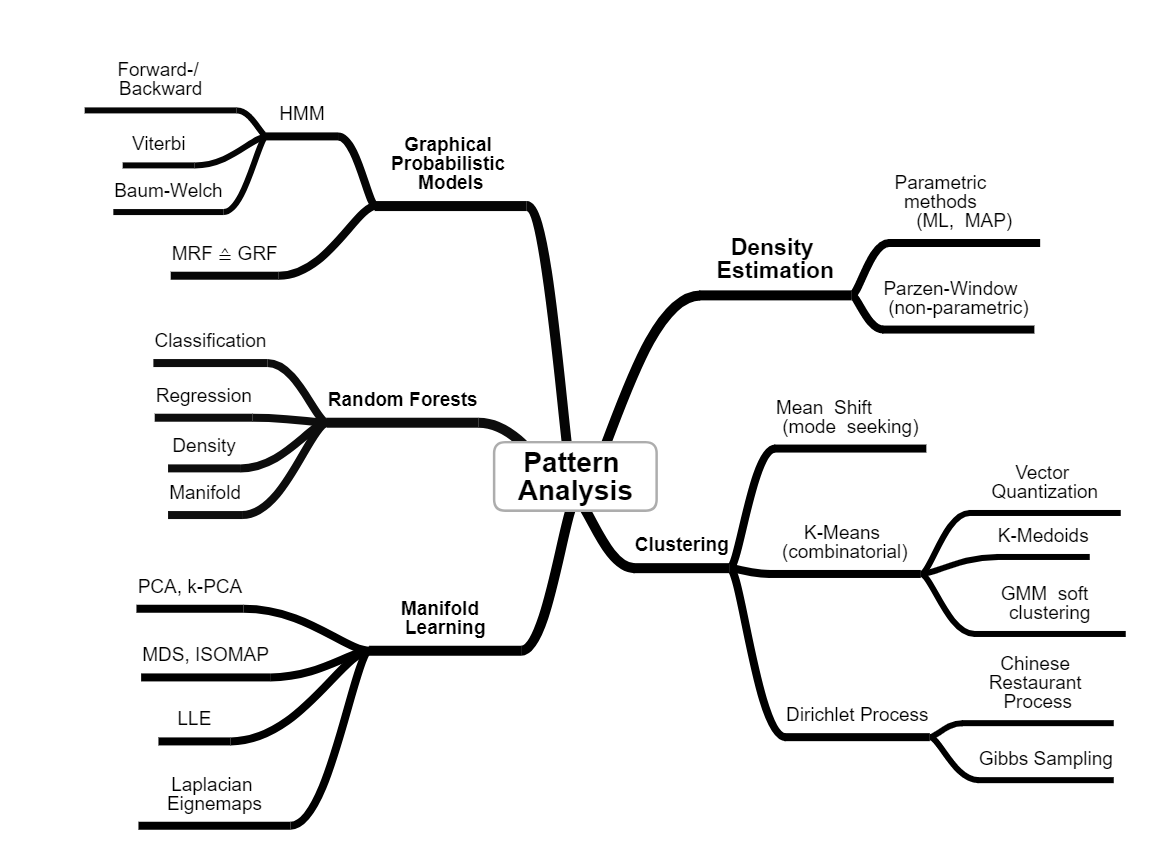
\includegraphics[width=\textwidth]{overview.png}
\end{titlepage}

{\centering
	This page is empty on purpose.\par
}

\newpage
\import{./src/}{density_estimation.tex}

\newpage
\import{./src/}{parzen_rosenblatt_estimator.tex}

\newpage
\import{./src/}{clustering.tex}

\newpage
\import{./src/}{mean_shift_algorithm.tex}

\newpage
\import{./src/}{k_means.tex}

\newpage
\import{./src/}{dirichlet_process.tex}

\newpage
\import{./src/}{manifold_learning.tex}

\newpage
\import{./src/}{k_pca.tex}

\newpage
\import{./src/}{multi_dimensional_scaling.tex}

\newpage
\import{./src/}{locally_linear_embedding.tex}

\newpage
\import{./src/}{laplacian_eigenmaps.tex}

\newpage
\import{./src/}{random_forest.tex}

\newpage
\import{./src/}{hidden_markov_model.tex}

\newpage
\import{./src/}{markov_random_fields.tex}

\end{document}
